\section{Methods Supplemental Information}

\subsection{Microwave Scattering}

The microwave scattering setup is shown in \ref{fig:SI_MWS_Setup_Silicon}. The parts were ordered from Erevant, formerly Sage Millimeter. The system is W-band and based on WR-10 waveguides. The microwave source is a 90 GHz Gunn oscillator (SOM-90305213-10-S1) with an output power of +13 dBm. The output of this source is fed into a 10 dB gain, +15 dBm P1dB, in-line waveguide power amplifier (SBP-7531141015-1010-E1). The output of the power amplifier is then fed into a 4-way in-line power divider (SWP-90310404-10-E1). In the current configuration, only two outputs of the power divider are used, and the remaining two are terminated with waveguide terminators (TODO). One power of the power divider is used for the main transmitted power, which is sent through waveguides to a horn (TODO) that transmits the microwaves into free space. The transmitted microwaves after the sample are collected by the same type of horn, and the collected microwaves are sent to the IQ mixer (SFQ-75311415-1010SF-N1-M). The LO input of the IQ mixer is fed by the remaining port of the power divider. Between the power divider and the LO input there is a phase shifter (STP-18-10-M2) that is typically used to maximize the I signal in the absence of a sample. 

The I and Q signals from the oscilloscope are fed directly into a Teledyne Leroy oscilloscope (TODO). The oscilloscope utilized 1 MOhm impedance. (TODO) The oscilloscope is triggered from the excimer laser. 

\begin{figure}[]
\centering
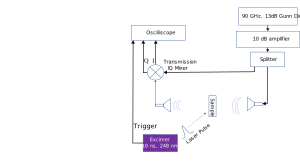
\includegraphics[width=0.8\textwidth]{\repodir/final/figures/SI/output/MWS_Setup.png}
\caption{Microwave scattering setup.}
\label{fig:SI_MWS_Setup}
\end{figure}

\begin{figure}[]
\centering
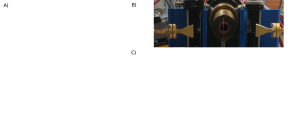
\includegraphics[width=0.8\textwidth]{\repodir/final/figures/SI/output/MWS_Silicon.png}
\caption{Silicon Measurements}
\label{fig:SI_MWS_Silicon}
\end{figure}

\begin{figure}[]
\centering
\includegraphics[width=0.8\textwidth]{\repodir/final/dataset/output/figures/mws_nothing_T0.png}
\caption{A) Measurement of transmission without any torch, B) position dependent transmission measurement.}
\label{fig:SI_MWS}
\end{figure}


\begin{figure}[]
\centering
\includegraphics[width=0.8\textwidth]{\repodir/final/dataset/output/figures/mws_nothing_time_trace_2023-05-18.png}
\caption{Time trace from 2023-05-18 of the transmission measurement without any free jet.}
\label{fig:SI_MWS}
\end{figure}

\ref{fig:SI_mws_processing_overview} shows the processing steps for the MWS data. 



\begin{figure}[]
\centering
\includegraphics[width=0.8\textwidth]{\repodir/experiment/analysis/mws/output/figures/mws_processing_overview.png}
\caption{Microwave processing overview}
\label{fig:SI_mws_processing_overview}
\end{figure}

\begin{figure}
\centering
\includegraphics[width=0.8\textwidth]{\repodir/experiment/analysis/mws/resampling/output/figures/mws_sample_nors_compare.png}
\caption{Comparison of the resampling methods.}
\label{fig:SI_mws_resampling}
\end{figure}


\begin{figure}
\centering
\includegraphics[width=0.8\textwidth]{\repodir/experiment/analysis/mws/output/figures/mws_fitting_compare.png}
\caption{Comparison of the fitting methods for the monomolecular regime. Fit to an exponential model and full solution of differential equation. }
\label{fig:SI_mws_fitting_compare}
\end{figure}

\clearpage
\subsection{Laser Profile}


\begin{figure}[H]
\centering
\includegraphics[width=0.8\textwidth]{\repodir/experiment/analysis/mws/output/figures/laser_profile.png}
\caption{Laser profile measurement}
\label{fig:SI_Laser_Profile}
\end{figure}

\clearpage
\subsection{AES}
\begin{figure}[]
    \centering
    \includegraphics[width=0.8\textwidth]{\repodir/experiment/analysis/absem/output/figures/absem_proc_overview.png}
    \caption{AES processing overview}
    \label{fig:SI_AES_proc_overview}
\end{figure}


\clearpage
\subsection{Emulsion Preparation and Delivery}

Potassium was introduced into the HVOF system by creating a potassium carbonate (K2CO3) brine and kerosene emulsion. This emulsion was delivered into the HVOF fuel flow via a tee. The tee run carried the fuel flow while the tee branch accepted emulsion through a PTFE feed line which was served by a high-pressure syringe pump. Three syringes were manifolded together. A switching valve allowed syringes to withdraw emulsion from the stirred reservoir or to infuse emulsion into the HVOF fuel line. Before, igniting the torch, the ?m emulsion line was filled. At the tee, fuel flow momentum was used to mix the emulsion with the fuel flow over the ?cm distance between the tee and combustion chamber nozzle. 


distributing brine droplets within part of the fuel supply via a water-in-oil emulsion (W/O). A droplet of W/O emulsion might be expected to pass through the combustor atomizer and promptly evaporate/burn from outer surface in. High surface to volume ratio, as well as close contact with the fuel should help the brine promptly evaporate, freeing the K2CO3 to dissociate, releasing gaseous, metallic potassium. To the extent the water boils after kerosene, water flashing to steam can break up kerosene droplets in the combustor and increase the effectiveness of mixing there. 

Literature was reviewed for an emulsion specifically designed to work with brine – especially water-in-oil (W/O) emulsions.  Developing emulsions for use in oilfields, Mohamed et al.\cite{mohamedInfluenceSurfactantStructure2017a} investigated high salinity W/O emulsions between “formation brine” and diesel. According to these authors, “[D]iesel and kerosene are used in the oilfields because of availability.” Their formation brine included more than 221,673 mg total dissolved solids (TDS) per liter of brine (~20% by mass).  

We noted the most stable result in ​[1]​ “reproduced” it using a potassium carbonate brine, kerosene, and a SPAN 80 / TWEEN 80 surfactant blend meeting their recommended HLB of 6.8. The concentration of the surfactant was 0.5% of the emulsion by volume - the minimum necessary found in [1] to obtain a stable emulsion. (Mohamed et al. measured ~5% of liquid came out of emulsion in 100 minutes at 120 °C).  

To generate the initial brine droplets, we used a spray nozzle. Spraying to create an emulsion is an age-old practice \cite{atkinsonKeroseneEmulsionHow1890} with relevance here because it avoids the temperature-rise associated with higher energy processes. These spray-generated droplets were then passed through an ultrasonic process to break them up further. This continuous process also minimized temperature rise because the material exited seconds after entering the ultrasonic field. 

The emulsion preparation process is given below:

Makes 500 mL 

1 . Prepare liquid components ahead of time 
\begin{itemize}
\item 100g supply of surfactant blend with HLB=6.8 by mixing 77g of Span 80 and 23g of Tween 80 on a magnetic stir plate 

\item Eight aliquots of K2CO3 brine by mixing 847.7g of K2CO3 powder into 350mL of deionized water on a magnetic stirrer 

\item Eight aliquots of prepared kerosene by mixing 5g of the surfactant blend into 106.5g of kerosene  

\item Each Brine/Kerosene aliquot pair will produce 500mL of emulsion. 
\end{itemize}


2. Prepare a 2-liter supply for a seeded firing experiment 

\begin{itemize}
    
\item Decant an aliquot of prepared kerosene into a beaker and begin stirring on a magnetic stir plate. 

\item Pump (peristaltic)the aliquot of K2CO3 brine through a spray nozzle, producing a mist of droplets to fall into the prepared kerosene. Droplet/kerosene interfaces adsorb the surfactant to make a relatively fine pre-emulsion. 

\item While continuing to magnetically stir, pump the pre-emulsion through an ultrasonic continuous flow cell to further break up the dispersed brine droplets. 

\item Batches were generally stored overnight and combined in magnetically stirred reservoir at the beginning of the photoionization experiment. 
\end{itemize}
